\documentclass[]{beamer}
\usepackage[T1]{fontenc}
\usepackage[utf8]{inputenc}
\usepackage[brazil]{babel} 
\setcounter{secnumdepth}{3}
\setcounter{tocdepth}{3}
\usepackage{amstext}
\usepackage{amssymb}
\usepackage[]{multicol}
\usepackage{graphicx}
\usepackage{fancybox}
\usepackage{mathtools,amssymb}
\usepackage{pgfplots}
\usepackage{tcolorbox}

\usepackage{pgf,tikz}
\usepackage{mathrsfs}
\usetikzlibrary{arrows}

\newcommand{\vv}{\overrightarrow}

\usepackage{tabto}
\usepackage{booktabs}
\usetheme{metropolis}

%fonte bacanuda para o texto
\usepackage[sfdefault]{FiraSans}
%fontes matemáticas profissionais
\usefonttheme{professionalfonts}
%%%%%%%%%%%%%%%%%%opções do metropolis
\metroset{titleformat=smallcaps}
\metroset{numbering=none}
\metroset{block=fill}


\definecolor{corcaqui}{RGB}{229,236,218}
\definecolor{coralerta}{RGB}{130,42,74}
\definecolor{corexemplo}{RGB}{111,190,182} %exemplo claro
\definecolor{verdeescuro}{RGB}{59,134,134}
\definecolor{corbloco}{RGB}{22,168,218}
\definecolor{corfundomarrom}{RGB}{68,36,29}
\definecolor{corfundoblocos}{RGB}{214,219,199}
\definecolor{corfundoalerta}{RGB}{246,191,194}
\definecolor{corfundoexemplo}{RGB}{186,223,205}
\definecolor{novobloco}{RGB}{142,135,106}


%\setbeamercolor{frametitle}{fg=white,bg=corfundomarrom}
\setbeamercolor{background canvas}{bg=corcaqui}
\setbeamercolor{block body}{bg=corfundoblocos}
\setbeamercolor{block title}{bg=novobloco}
\setbeamercolor{block title alerted}{bg=coralerta}
\setbeamercolor{block title example}{bg=verdeescuro}
\setbeamercolor{alerted text}{fg=white}
\setbeamercolor{example text}{fg=white}
\setbeamercolor{block body alerted}{bg=corfundoalerta}
\setbeamercolor{block body example}{bg=corfundoexemplo}

\newcommand{\rr}{\mathbb{R}}
\DeclarePairedDelimiter{\abs}{\lvert}{\rvert}


%%%%%%%%%%%%%%%%%%%%%%%%%%%%%%       Slide      %%%%%%%%%%%%%%%%%%%%%%%%%%%%%%%%%%%%%%%%
\begin{document}


\begin{frame}[t]{\centering Universidade Federal de Jataí}

  
\begin{center}
  \textsc{\huge{Tudo o que eu queria que alguém me falasse
      \textcolor{red}{(não só sobre Matemática)} quando eu era jovem}}
  \end{center}
  

\end{frame}

%%%%%%%%%%%%%%%%%%%%%%%%%%%%%%       Slide      %%%%%%%%%%%%%%%%%%%%%%%%%%%%%%%%%%%%%%%%

\begin{frame}{Em resumo}

\begin{tcolorbox}[
  colback=black!10!white, % color fundo do texto. preto 10%, depois branco
  colframe=black!70!white, % color do título e em volta)
  colupper=red!75!black, % cor da fonte de cima
  collower=blue!75!black, % cor da fonte de baixo
  title= Ninguém vai saber Matemática pra você]
  Grandes empresas, bancos e políticos podem contratar quem
  sabe Matemática e tirar vantagem sobre você:
  \tcblower
  \begin{itemize}
  \item Compras parceladas
  \item Planos de telefonia
  \item Produtos com quantidade maquiada
  \item Financiamentos
  \item Garantia extendida
  \item Fazendo você, basicamente, dar uma quantidade de dinheiro que você
    acha que não tem, de graça,
    por nada!
  \end{itemize}
\end{tcolorbox}
  



\end{frame}

%%%%%%%%%%%%%%%%%%%%%%%%%%%%%% Slide      %%%%%%%%%%%%%%%%%%%%%%%%%%%%%%%%%%%%%%%%

\begin{frame}{Usando a função exponencial a seu favor}

\begin{tikzpicture}
  \node [fill=corfundoblocos, rounded corners=5pt] { 
    \begin{minipage}{1.0\textwidth}
Se você não entende como funciona \textbf{na prática} a \\ função exponencial, vai literalmente pagar caro!
    \end{minipage} };
\end{tikzpicture} 


\begin{center}
$f(x)=e^x$
\end{center}


\begin{tikzpicture}
  \node [fill=corfundoblocos, rounded corners=5pt] { 
    \begin{minipage}{1.0\textwidth}
Veremos agora como \textbf{parece} que economizar pouco dinheiro não vale a pena, mas se você realmente entender a função \\ exponencial, vai saber que sempre vale a pena!
    \end{minipage} };
\end{tikzpicture} 


\end{frame}


%%%%%%%%%%%%%%%%%%%%%%%%%%%%%% Slide      %%%%%%%%%%%%%%%%%%%%%%%%%%%%%%%%%%%%%%%%

\begin{frame}{Exponencial na prática: Comprando um carro}

\begin{tikzpicture}
\node [fill=lightgray, rounded corners=5pt] { 
\begin{minipage}{1.0\textwidth}
Suponha que você queira comprar um automóvel
de $R\$ 21.589,42$, financiado em 60 meses a juros de $0,6\%$ ao mês.
Esta é uma boa taxa, mas você pagaria prestações de $R\$ 429,54$ e no
final do período desembolsaria $R\$ 25.772,40$.
\end{minipage} };
\end{tikzpicture}

\pause{}

\begin{tikzpicture}
\node [fill=cyan!40, rounded corners=5pt] { 
\begin{minipage}{1.0\textwidth}
Suponha que em vez disso, você resolvesse
colocar $R\$ 300,00$ por mês na poupança, rendendo aproximadamente $0,6\%$
mensalmente. Em em cinco anos acumularia os mesmos $R\$ 21.589,42$. 
\end{minipage} };
\end{tikzpicture}

\pause{}

\begin{tikzpicture}
\node [fill=gray!50, rounded corners=5pt] { 
\begin{minipage}{1.0\textwidth}
A soma dos depósitos nesses sessenta meses seria
de $R\$ 18.000,00$, mas os juros do banco teriam trabalhado para você
e viabilizariam a compra de um automóvel melhor. Desta forma, os juros
trabalhariam a seu favor, e não contra!
\end{minipage} };
\end{tikzpicture}

\end{frame}

%%%%%%%%%%%%%%%%%%%%%%%%%%%%%% Slide      %%%%%%%%%%%%%%%%%%%%%%%%%%%%%%%%%%%%%%%%

\begin{frame}{O problema com a Caderneta de Poupança}

\begin{tikzpicture}
  \node [fill=lightgray, rounded corners=5pt] { 
    \begin{minipage}{1.0\textwidth}
O cálculo da rentabilidade da poupança está sempre sujeito a alterações e pode ser que o rendimento da poupança fique abaixo da inflação.
    \end{minipage} };
\end{tikzpicture}

\pause

Caso isso aconteça, um título de renda fixa indexada à
inflação pode ser melhor. Mas e as taxas? E a liquidez? (nem
sempre uma aplicação fornece o dinheiro na hora que
queremos!)

\pause

\begin{tikzpicture}
  \node [fill=red!40, rounded corners=5pt] { 
    \begin{minipage}{1.0\textwidth}
Você não tem escolha: você precisa estudar para saber o que é melhor pra você, não deixe que decidam por você!
    \end{minipage} };
\end{tikzpicture} 



\end{frame}

%%%%%%%%%%%%%%%%%%%%%%%%%%%%%% Slide %%%%%%%%%%%%%%%%%%%%%%%%%%%%%%%%%

\begin{frame}{O que acontece com o dinheiro na poupança}

\begin{center}
\begin{tabular}{|c|c|c|c|}
\hline 
Mês & Depósito & Acumulado & Juro ac.\tabularnewline
\hline 
\hline 
1 & 300,00 & 300,00 & 0,00\tabularnewline
\hline 
2 & 300,00 & (300{*}1,006)+300=601,8 & 1,80\tabularnewline
\hline 
3 & 300,00 & (601,8{*}1,006)+300=905,41 & 5,41\tabularnewline
\hline 
4 & 300,00 & ~~~(905,41{*}1,006)+300=1210,84~~~~ & ~~10,84~~\tabularnewline
\hline 
\end{tabular}
\par\end{center}

\begin{center}
$\cdots$
\par\end{center}

\begin{center}
\begin{tabular}{|c|c|c|c|}
\hline 
~~58~ & ~~300,00~ & (20016,12{*}1,006)+300=20738,02 & 3338,02\tabularnewline
\hline 
~~59~ & ~~300,00~ & (20738,02{*}1,006)+300=21162,44 & 3462,44\tabularnewline
\hline 
~~60~ & ~~300,00~ & (21162,44{*}1,006)+300=21589,42 & 3589,42\tabularnewline
\hline 
\end{tabular}
\par\end{center}

\end{frame}

%%%%%%%%%%%%%%%%%%%%%%%%%%%%%%       Slide      %%%%%%%%%%%%%%%%%%%%%%%%%%%%%%%%%%%%%%%%

\begin{frame}{O segredo dos juros compostos}

\begin{tikzpicture}
\node [fill=cyan, rounded corners=5pt] { 
\begin{minipage}{1.0\textwidth}
Os juros compostos funcionam em um modelo exponencial.
A função exponencial cresce mais rápido quanto maior o valor de x,
por isso se diz que ``juro de muito é muito, juro de pouco é pouco''.
\end{minipage} };
\end{tikzpicture}

\large {O curso de Cálculo estuda as funções que são utilizadas neste momento.
Se não forem utilizadas por você, certamente serão pelos bancos!}

\end{frame}

%%%%%%%%%%%%%%%%%%%%%%%%%%%%%%       Slide      %%%%%%%%%%%%%%%%%%%%%%%%%%%%%%%%%%%%%%%%

\begin{frame}{Mais um exemplo}

\begin{tikzpicture}
\node [fill=yellow, rounded corners=5pt] { 
\begin{minipage}{1.0\textwidth}
Após 1 ano investindo R\$ 100,00/mês com rentabilidade de 1\% ao mês,
você terá R\$ 1.268,25, ou seja, somente R\$ 68,25 de ganhos.
\end{minipage} };
\end{tikzpicture}

\pause{}

\begin{tikzpicture}
\node [fill=orange, rounded corners=5pt] { 
\begin{minipage}{1.0\textwidth}
Pode parecer pouco resultado para muito esforço, mas depois de 120 meses (ou 10 anos), você terá
R\$ 23.003,87 e terá investido, de fato, R\$ 12.000,00, ou seja, já
conta com um lucro de R\$ 11.003,87, quase o dobro do valor investido. 
\end{minipage} };
\end{tikzpicture}

\pause{}

\begin{tikzpicture}
\node [fill=red, rounded corners=5pt] { 
\begin{minipage}{1.0\textwidth}
Após 20 anos (240 meses), terá R\$ 98.925,54, após 30 anos terá R\$
349.496,41 e após 40 anos R\$ 1.176.477,25 contra R\$ 48.000,00 aplicados.
\end{minipage} };
\end{tikzpicture}
\end{frame}

%%%%%%%%%%%%%%%%%%%%%%%%%%%%%%       Slide      %%%%%%%%%%%%%%%%%%%%%%%%%%%%%%%%%%%%%%%%

\begin{frame}{\foreignlanguage{brazil}{Fórmulas utilizadas}}

\begin{center}
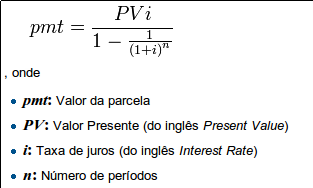
\includegraphics[scale=0.5]{price}
\par\end{center}

\begin{center}
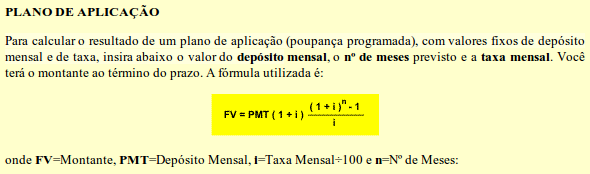
\includegraphics[scale=0.55]{poupprog}
\par\end{center}

\end{frame}

%%%%%%%%%%%%%%%%%%%%%%%%%%%%%%%%%%%% slide %%%%%%%%%%%%%%%%%%%%%%%%%

\begin{frame}[standout]{Dicas além da função exponencial }

\end{frame}



%%%%%%%%%%%%%%%%%%%%%%%%%%%%%%       Slide      %%%%%%%%%%%%%%%%%%%%%%%%%%%%%%%%%%%%%%%%
\begin{frame}{Compras parceladas}

  \begin{itemize}
    \item Todos vão fazer o máximo para que você se
      concentre apenas no valor da parcela e não no valor
      total. Muito, muito cuidado e jamais se esqueça disso:
      o que importa é o valor total com juros e não a
      parcela.
      \pause
\item As operadoras de cartão sabem do poder da função
  exponencial, mas claro: usam a favor delas!
\item Nunca parcele com juros: você estará dando dinheiro de
  graça por nada!
  \pause
\item Caso você consiga se planejar e economizar antes, pode
  conseguir negociar um desconto à vista. \textbf{É assim que se faz negócio.}
\end{itemize}

\end{frame}
%%%%%%%%%%%%%%%%%%%%%%%%%%%%%%       Slide      %%%%%%%%%%%%%%%%%%%%%%%%%%%%%%%%%%%%%%%%
\begin{frame}{Planos de telefonia. Planos em geral}
  \begin{itemize}
  \item O plano é pra operadora, nunca pra você.
    \pause
    \item As operadoras não tem vergonha de fazer propostas
      absurdamente ruins para seus clientes: fica a cargo
      exclusivamente seu avaliar se vale a pena ou não - e
      as operadoras ganham por cansaço com a burocracia que
      pode ser proposital e a pessoa perde a
      paciência fazer as contas ou de
      ler parágrafos grandes assim e
      simplesmente assina.
      \pause
    \item Os planos são propositalmente nebulosos e a única
      coisa que pode barrar isso é a lei, que explorada na
      margem, no limite!
    \end{itemize}
    \pause

    \begin{tikzpicture}
      \node [fill=red!50, rounded corners=5pt] { 
        \begin{minipage}{1.0\textwidth}
          Ou você estuda por você mesmo, ou alguém tira proveito de você.
        \end{minipage} };
    \end{tikzpicture} 

    
  \end{frame}
%%%%%%%%%%%%%%%%%%%%%%%%%%%%%%       Slide      %%%%%%%%%%%%%%%%%%%%%%%%%%%%%%%%%%%%%%%%
  \begin{frame}{Produtos maquiados}

    \begin{itemize}
    \item Você já deve ter ouvido a história do tamanho do
      buraco do tubo da pasta de dentes. A ideia é sempre
      não retirar o máximo de dinheiro do cliente.
      \pause
      \item Por que açolgue e padaria ficam no final do supermercado?
        Porque vendem produtos que são consumidos rápido,
        logo você precisará voltar e passará antes por todos
        os outros produtos.
        \pause
      \item O vendedor de uma loja (geralmente o dono) quer
        fazer o melhor negócio pra ele. Observe que o que
        ele te oferece primeiro nem sempre tem a ver com o
        que você quer, é apenas o que ele quer vender.
        \pause
      \item Vc já viu produtos de 800g no supermercado. Eram
        de 1kg. Começaram a aparecer produtos de 380g. Eram
        de meio kg. Uma marca que faz isso quer tirar
        proveito do cliente.
    \end{itemize}

\end{frame}
%%%%%%%%%%%%%%%%%%%%%%%%%%%%%%       Slide      %%%%%%%%%%%%%%%%%%%%%%%%%%%%%%%%%%%%%%%%
\begin{frame}{Garantia extendida}
\begin{itemize}
\item Os produtos, que antes eram feitos de material bom,
  hoje são feitos de qualquer material, mas determinados
  produtos e marcas ainda tem um bom controle de qualidade.
  \pause
  \item Quando a marca do produto coloca um prazo de
    garantia, ela quer ter certeza que não terá problemas e
    coloca um prazo que sabe que não dará problemas.
    \pause
  \item Se aproveitando disso, várias grandes redes querem
    te vender garantia extendida da própria loja, que quase
    nunca é utilizada. Ou seja: você dá seu dinheiro de
    graça, por nada!
\end{itemize}

\end{frame}

%%%%%%%%%%%%%%%%%%%%%%%%%%%%%% Slide      %%%%%%%%%%%%%%%%%%%%%%%%%%%%%%%%%%%%%%%%
\begin{frame}{Leia as intruções}
  \begin{itemize}
  \item Manuais de instrução não estão lá apenas para o
    cliente se informar sobre o produto. Estão lá para
    evitar que a empresa perca eventuais processos
    judiciais.
    \item É dever seu, como cliente, se informar sobre o que
      está comprando. Ninguém vai fazer isso pra você. Na
      bula, nas letras miúdas, estão todas as informações
      que você deve saber.
\item Nunca assine nada sem ler tudo
  \end{itemize}

\end{frame}
%%%%%%%%%%%%%%%%%%%%%%%%%%%%% Slide %%%%%%%%%%%%%%%%%%%%%%%%%%%%%%%%%%%%
\begin{frame}{Financiamentos}
\begin{itemize}
\item Todo financiamento é muito melhor para a instituição
  financeira do que pra você. MUITO melhor.
\item As instituições financeiras sabem como extrair de você
  uma quantidade de dinheiro que você acha que não tem,
  porque você olha apenas para o que tem no momento.
  \pause
  \item Mas agora você já sabe que a função exponencial
    (juros, poupança) depende mais do tempo que da
    quantidade de dinheiro que você tem no momento.
    \pause
  \item A realidade é que a grande maioria de nós precisa de
    financiamento, porque economizar não faz parte da
    cultura do brasileiro.
    \pause
  \item Ao fazer um financiamento, prepare-se para
    economizar o máximo que puder e conversar com o gerente
    para \textbf{abater direto no saldo devedor}

\end{itemize}
\end{frame}
%%%%%%%%%%%%%%%%%%%%%%%% slide %%%%%%%%%%%%%%%%%%%%

\begin{frame}{Pagar parcelas sempre é ruim}

  \begin{itemize}
  \item Em geral, apenas $30\%$ de uma parcela é abatida da
    sua dívida. O restante é dinheiro que você dá, de graça.
    \pause
  \item Economize, estude, vá ao banco e peça abatimento do
    saldo devedor.
    \pause
    \item Os bancos podem te pedir para esperar ou voltar
      outro dia, porque, você sabe, computadores demoram
      muito pra fazer contas (sqn).
      \pause
    \item Nesse tempo, podem te oferecer outras alternativas
      de investimento, mas você nunca conseguirá ganhar mais
      do que paga ao banco em juros.
      \pause
    \item Outro argumento constante: mas todo mundo usa esse
      modelo de juros, por que você quer usar este outro??
      \pause
    \item Quando te perguntarem se você quer diminuir a
      parcela ou o tempo do financiamento, escolha diminuir
      a parcela, porque assim você consegue economizar mais.
  \end{itemize}

\end{frame}

%%%%%%%%%%%%%%%%%%%%%%%%%%%%%%%% slide %%%%%%%%%%%%%%%%%%%%

\begin{frame}{Aluguel ou financiamento}

\begin{itemize}
\item É comum pensar que ao fazer um financiamento estamos
  ``pagando pelo que é nosso'' enquanto no aluguel jogamos
  dinheiro fora.
  \pause
\item Mas faça as contas \textbf{você mesmo}. Não é raro que
  pagar um aluguel barato seja melhor que pagar um
  financiamento.
\item Se você conseguir economizar dinheiro com um aluguel
  barato, os juros, a função exponencial, vai trabalhar a
  seu favor.
\item Pagando um financiamento, a função exponencial
  trabalha a favor dos bancos (e eles sabem usar isso muito
  bem).
  \pause
\item Raramente o financiamento vai ser melhor que o alguel.
\end{itemize}
  
\end{frame}
%%%%%%%%%%%%%%%%%%%%%%%%%%%%%%%%%%% slide %%%%%%%%%%%%%%%%%%%%%%

\begin{frame}{Seu computador, seu celular, não são seus}

  \begin{itemize}
  \item Você paga por eles, mas as empresas usam mais que
    você, e tem preferência.
  \item Seu computador e celular atendem primeiro as grandes
    empresas e \textbf{se der} te atendem depois.
    \pause
  \item A página de internet carrega devagar pq carrega
    anúncios primeiro. Se você não paga, você é o produto. E
    por aí vai a internet...
  \item É impossível escapar, mas tentem usar
    duckduckgo.com, Manjaro Linux e evitem redes sociais.
    \pause
  \item  Estas últimas serão usadas contra nós, mas fazem parte
    da vida moderna.
  \end{itemize}

\end{frame}

%%%%%%%%%%%%%%%%%%%%%%%%%%%%%%       Slide      %%%%%%%%%%%%%%%%%%%%%%%%%%%%%%%%%%%%%%%%
  \begin{frame}{Plano de ação}

    \begin{enumerate}
    \item Estude. Nem seus pais podem fazer isso pra você. \pause
    \item Planeje.\pause
    \item Eliminar dívidas é sempre a primeira coisa.\pause
    \item Priorize qualidade de vida e economia em cada
      compra. É assim que se guarda dinheiro.\pause
    \item Depois que eliminar as dívidas, contrua uma
      poupança equivalente a 3 meses de salário, que você
      usará apenas em emergências.\pause
    \item Sim, eu sei que é difícil e parece impossível. Pra
      mim também é, mas eu assisti e li Naruto.\pause
    \item Pense em garantir sua aposentadoria sem precisar
      da aposentadoria do governo (não conte com ela)
    \end{enumerate}

   \end{frame} 


%%%%%%%%%%%%%%%%%%%%%%%%%%%%%%       Slide      %%%%%%%%%%%%%%%%%%%%%%%%%%%%%%%%%%%%%%%%
\begin{frame}[standout]{As empresas não são o pior}

  se vc acha que empresas são más por usarem a borda da lei para se
  aproveitar de clientes, não se assuste: políticos, partidos e sistemas
  político-econômicos (quaquer um) são muito piores. Não confie em nenhum deles. 
\end{frame}


%%%%%%%%%%%%%%%%%%%%%%%%%%%%%%       Slide      %%%%%%%%%%%%%%%%%%%%%%%%%%%%%%%%%%%%%%%%
\begin{frame}{Dica divertida, mas séria}

  \textbf{\Huge{Assistam Naruto e aprendam com ele e o Maito
    Gai}}

\end{frame}

%%%%%%%%%%%%%%%%%%%%%%%%%%%%%%       Slide      %%%%%%%%%%%%%%%%%%%%%%%%%%%%%%%%%%%%%%%%



%%%%%%%%%%%%%%%%%%%%%%%%%%%%%%       Slide      %%%%%%%%%%%%%%%%%%%%%%%%%%%%%%%%%%%%%%%%



%%%%%%%%%%%%%%%%%%%%%%%%%%%%%%       Slide      %%%%%%%%%%%%%%%%%%%%%%%%%%%%%%%%%%%%%%%%



%%%%%%%%%%%%%%%%%%%%%%%%%%%%%%       Slide      %%%%%%%%%%%%%%%%%%%%%%%%%%%%%%%%%%%%%%%%


%%%%%%%%%%%%%%%%%%%%%%%%%%%%%%       Slide      %%%%%%%%%%%%%%%%%%%%%%%%%%%%%%%%%%%%%%%%



%%%%%%%%%%%%%%%%%%%%%%%%%%%%%%       Slide      %%%%%%%%%%%%%%%%%%%%%%%%%%%%%%%%%%%%%%%%



%%%%%%%%%%%%%%%%%%%%%%%%%%%%%%       Slide      %%%%%%%%%%%%%%%%%%%%%%%%%%%%%%%%%%%%%%%%



%%%%%%%%%%%%%%%%%%%%%%%%%%%%%%       Slide      %%%%%%%%%%%%%%%%%%%%%%%%%%%%%%%%%%%%%%%%


%%%%%%%%%%%%%%%%%%%%%%%%%%%%%%       Slide      %%%%%%%%%%%%%%%%%%%%%%%%%%%%%%%%%%%%%%%%



%%%%%%%%%%%%%%%%%%%%%%%%%%%%%%       Slide      %%%%%%%%%%%%%%%%%%%%%%%%%%%%%%%%%%%%%%%%



%%%%%%%%%%%%%%%%%%%%%%%%%%%%%%       Slide      %%%%%%%%%%%%%%%%%%%%%%%%%%%%%%%%%%%%%%%%



%%%%%%%%%%%%%%%%%%%%%%%%%%%%%%       Slide      %%%%%%%%%%%%%%%%%%%%%%%%%%%%%%%%%%%%%%%%


%%%%%%%%%%%%%%%%%%%%%%%%%%%%%%       Slide      %%%%%%%%%%%%%%%%%%%%%%%%%%%%%%%%%%%%%%%%



%%%%%%%%%%%%%%%%%%%%%%%%%%%%%%       Slide      %%%%%%%%%%%%%%%%%%%%%%%%%%%%%%%%%%%%%%%%



%%%%%%%%%%%%%%%%%%%%%%%%%%%%%%       Slide      %%%%%%%%%%%%%%%%%%%%%%%%%%%%%%%%%%%%%%%%



%%%%%%%%%%%%%%%%%%%%%%%%%%%%%%       Slide      %%%%%%%%%%%%%%%%%%%%%%%%%%%%%%%%%%%%%%%%


%%%%%%%%%%%%%%%%%%%%%%%%%%%%%%       Slide      %%%%%%%%%%%%%%%%%%%%%%%%%%%%%%%%%%%%%%%%



%%%%%%%%%%%%%%%%%%%%%%%%%%%%%%       Slide      %%%%%%%%%%%%%%%%%%%%%%%%%%%%%%%%%%%%%%%%



%%%%%%%%%%%%%%%%%%%%%%%%%%%%%%       Slide      %%%%%%%%%%%%%%%%%%%%%%%%%%%%%%%%%%%%%%%%



%%%%%%%%%%%%%%%%%%%%%%%%%%%%%%       Slide      %%%%%%%%%%%%%%%%%%%%%%%%%%%%%%%%%%%%%%%%


%%%%%%%%%%%%%%%%%%%%%%%%%%%%%%       Slide      %%%%%%%%%%%%%%%%%%%%%%%%%%%%%%%%%%%%%%%%



%%%%%%%%%%%%%%%%%%%%%%%%%%%%%%       Slide      %%%%%%%%%%%%%%%%%%%%%%%%%%%%%%%%%%%%%%%%



%%%%%%%%%%%%%%%%%%%%%%%%%%%%%%       Slide      %%%%%%%%%%%%%%%%%%%%%%%%%%%%%%%%%%%%%%%%



%%%%%%%%%%%%%%%%%%%%%%%%%%%%%%       Slide      %%%%%%%%%%%%%%%%%%%%%%%%%%%%%%%%%%%%%%%%




%%%%%%%%%%%%%%%%%%%%%%%%%%%%%%       Slide      %%%%%%%%%%%%%%%%%%%%%%%%%%%%%%%%%%%%%%%%


%%%%%%%%%%%%%%%%%%%%%%%%%%%%%%       Slide      %%%%%%%%%%%%%%%%%%%%%%%%%%%%%%%%%%%%%%%%



%%%%%%%%%%%%%%%%%%%%%%%%%%%%%%       Slide      %%%%%%%%%%%%%%%%%%%%%%%%%%%%%%%%%%%%%%%%



%%%%%%%%%%%%%%%%%%%%%%%%%%%%%%       Slide      %%%%%%%%%%%%%%%%%%%%%%%%%%%%%%%%%%%%%%%%



%%%%%%%%%%%%%%%%%%%%%%%%%%%%%%       Slide      %%%%%%%%%%%%%%%%%%%%%%%%%%%%%%%%%%%%%%%%


%%%%%%%%%%%%%%%%%%%%%%%%%%%%%%       Slide      %%%%%%%%%%%%%%%%%%%%%%%%%%%%%%%%%%%%%%%%



%%%%%%%%%%%%%%%%%%%%%%%%%%%%%%       Slide      %%%%%%%%%%%%%%%%%%%%%%%%%%%%%%%%%%%%%%%%



%%%%%%%%%%%%%%%%%%%%%%%%%%%%%%       Slide      %%%%%%%%%%%%%%%%%%%%%%%%%%%%%%%%%%%%%%%%



%%%%%%%%%%%%%%%%%%%%%%%%%%%%%%       Slide      %%%%%%%%%%%%%%%%%%%%%%%%%%%%%%%%%%%%%%%%


%%%%%%%%%%%%%%%%%%%%%%%%%%%%%%       Slide      %%%%%%%%%%%%%%%%%%%%%%%%%%%%%%%%%%%%%%%%



%%%%%%%%%%%%%%%%%%%%%%%%%%%%%%       Slide      %%%%%%%%%%%%%%%%%%%%%%%%%%%%%%%%%%%%%%%%



%%%%%%%%%%%%%%%%%%%%%%%%%%%%%%       Slide      %%%%%%%%%%%%%%%%%%%%%%%%%%%%%%%%%%%%%%%%



%%%%%%%%%%%%%%%%%%%%%%%%%%%%%%       Slide      %%%%%%%%%%%%%%%%%%%%%%%%%%%%%%%%%%%%%%%%


%%%%%%%%%%%%%%%%%%%%%%%%%%%%%%       Slide      %%%%%%%%%%%%%%%%%%%%%%%%%%%%%%%%%%%%%%%%



%%%%%%%%%%%%%%%%%%%%%%%%%%%%%%       Slide      %%%%%%%%%%%%%%%%%%%%%%%%%%%%%%%%%%%%%%%%



%%%%%%%%%%%%%%%%%%%%%%%%%%%%%%       Slide      %%%%%%%%%%%%%%%%%%%%%%%%%%%%%%%%%%%%%%%%



%%%%%%%%%%%%%%%%%%%%%%%%%%%%%%       Slide      %%%%%%%%%%%%%%%%%%%%%%%%%%%%%%%%%%%%%%%%




\end{document}
